\documentclass[11pt, leqno]{article}
\usepackage[margin=0.5in]{geometry}
\usepackage{amsfonts,amsmath,amssymb,amsthm}
\usepackage{ragged2e}
\usepackage{graphicx}
\author{Nikolai Merritt}
\title{Understanding Calculus for Beginners}
\date{\vspace{-5ex}}
\numberwithin{equation}{section}
\graphicspath{{Images/}}

\begin{document}
\newcommand{\D}[2]{\frac{\text{d}#1}{\text{d}#2}}
\newcommand{\asreq}{\textrm{, as required.}}
\maketitle

\newpage
\tableofcontents

\newpage
\section{Know your Limits}
Imagine that you're watching a live game of basketball, on your TV. Your favourite team's been playing well, but there's only half a minute left, and they're just one point behind. Their lead player gets the ball, spotting a clear path to the opposition's net. He throws the ball towards it as you sit on the edge of your seat, staring intently at the TV screen. Halfway as the ball curves through the air, the connection stutters for a split second, but when it resumes the ball has fallen through the net, and your favourite team's cheering. 
\\ \\
Now, even though you never actually saw what happened in those last few seconds of the game, it doesn't take a genius to figure it out. Just before the connection stuttered, it was looking like the ball was going to fall through the hoop. And, immediately after the connection stuttered, it looked like the ball fell through the hoop too. In fact, if you replayed the last thirty seconds of the match in slow motion, you'd observe that as the time gets closer and closer to the bit where the connection was lost, the ball gets closer and closer to falling into the hoop. And, the closer and closer we get to immediately after the connection was lost, the clearer and clearer it is that the ball fell through the hoop too. So, while you haven't seen for your own eyes what happened at that time, you can still have an incredibly accurate idea of what went on.  
\\ \\
This very intuitive way of thinking can be applied not only to everyday life, but to great effect in mathematics too. Imagine that Jim is in charge of monitoring the daily water level at the river Thames, and it so happens that the rise of millimetres of water height, in terms of times passed in hours, is
\begin{align*}
\text{rise in water level} &= \frac{(t + 5) \ (t - 12)}{t - 12}.
\end{align*}
\\ \\
If Jim called us 8 hours in and asked us how what the rise in water level was, we could simply put 8 into our formula to get:
\begin{align*}
\text{rise in water level} &= \frac{(8 + 5) \ (8 - 12)}{8 - 12} = \frac{13 \times -4}{-4} = 13 \ \text{mm.}
\end{align*}
\\ \\ 
But here's the problem: what if Jim then wanted us to check the rise 12 hours in? Simply putting 12 into our formula would give us:
\begin{align*}
\text{rise in water level} = \frac{(12 + 5) \ (12 - 12)}{12 - 12} = \frac{17 \times 0}{0}.
\end{align*}
And we don't know the answer to this question. No one knows what anything divided by zero is. 
\\ \\
However, we can still offer Jim an incredibly good estimate to how much the Thames' water level has risen. Like in our earlier basketball scenario, we can look at what happens when the time passed gets closer and closer to 12 and make a guess from that. \(t = 11.5\) seems to be as good a start as any:
\begin{align*}
\text{rise in water level} = \frac{(11.5 + 5) \ (11.5 - 12)}{11.5 - 12} = \frac{16.5 \times -0.5}{-0.5} = 16.5 \, \text{mm.}
\end{align*}
\\ Now let's get closer. \(t = 11.9\) will give us a more accurate guess:
\begin{align*}
\text{rise in water level} = \frac{(11.9 + 5) \ (11.9 - 12)}{11.9 - 12} = \frac{16.9 \times -0.1}{-0.1} = 16.9 \, \text{mm.}
\end{align*}
\\ And if we wanted to get even more accurate still, when \(t = 11.999\):
\begin{align*}
\text{rise in water level} = \frac{(11.999 + 5) \ (11.999 - 12)}{11.999 - 12} = \frac{16.999 \times -0.0001}{-0.0001} = 16.999 \ \text{mm.}
\end{align*}
\\ Just to be sure, let's check the water level rise immediately after 12 minutes. If everything goes well, this should give us an answer very close to 17 too:
\begin{align*}
\text{rise in water level} = \frac{(12.0001 + 5) \ (12.0001 - 12)}{12.0001 - 12} = \frac{17.0001 \times 0.0001}{0.0001} = 17.0001 \, \text{mm.}
\end{align*}
\\ So we can safely say that, as the time passed gets closer and closer to 12 minutes, our answer gets closer and closer to 17 mm. In other words, the approaching value of our water level rise is 17, as \(t\) approaches 12.
\\ For whatever reason, mathematicians use the word ``limiting" instead of ``approaching". They'd say that the \textbf{limiting value} -- or ``limit" for short -- of our answer is 17, as \(t\) gets closer to 12.
\\ \\ Because the idea of finding a limit is such a useful tool, mathematicians have also invented their own notation for it. Instead of having to write out the previous sentence, they would write:
\begin{flalign*}
\lim_{t \to 12} \left( \text{rise in water level} \right) = 17 \\
\intertext{or } \lim_{t \to 12} \frac{(t+5) \ (t - 12)}{t-12} = 17.
\end{flalign*}
\\ Now that we've got the jargon out the way, you may be wondering how we can be so sure our limit is 17 \textit{exactly}? What if our rise actually approaches, say, 16.9998, 17.0002, or 17 \( + \frac{2}{8653}\)? While our answer of ``some number pretty damn close to 17" should do just fine for this simple scenario, knowing if some function limits to, say, \(\pi\), with all its uses and shortcuts, instead of 3.1416, can be vital for more important situations. This is why most limits are solved algebraically, instead of plugging in numbers and watching what happens. This allows for far more precision and rigour.  
\\ \\ Thankfully, just like how fundamentally simple the idea of a limit is, so are the ways in which it can be used. Unlike a concrete function like \(\sin(x)\), a limit is more like a concept, and so is a bit more malleable. When we're adding, subtracting, multiplying or dividing different functions, it doesn't matter whether we look at what they approach together, or considered individually; it makes no difference to our answer. Or, in mathematical terms...
\begin{flalign*}
\intertext{For any functions \(f(x)\) and \(g(x)\), and any number \(c\), }
\lim_{x \to c} \left[ f(x) + g(x) \right] &= \lim_{x \to c} f(x) \ + \ \lim_{x \to c} g(x) \\ \\
\lim_{x \to c} \left[ f(x) - g(x) \right] &= \lim_{x \to c} f(x) \ - \ \lim_{x \to c} g(x) \\ \\
\lim_{x \to c} \left[ f(x) \times g(x) \right] &= \lim_{x \to c} f(x) \ \times \ \lim_{x \to c} g(x) \\ \\
\lim_{x \to c} \, \frac{f(x)}{g(x)} &= \frac{\lim\limits_{x \to c} f(x)}{\lim\limits_{x \to c} g(x)}
\end{flalign*}
\\ With these four properties made clear, we can easily start to demonstrate how we could work out the limit for our water level equation algebraically:
\begin{align*}
\lim_{t \to 12} \frac{(t + 5) \ (t - 12)}{t - 12} &= \lim_{t \to 12} \left( \frac{t - 12}{t - 12} \ (t + 5) \right) \\ \\
 &= \lim_{t \to 12} \left(\frac{t - 12}{t - 12}\right) \times \lim_{t \to 12} (t + 5).
\end{align*}
\\ Note that we're taking the limit as \(t\) approaches 12. Similar to our estimation in the mystery connection loss in our basketball scenario, we see what happens as \(t\) \textit{approaches} 12, not when \(t\) \textit{is} 12 So, cancelling both sides of the fraction won't be dividing by zero. This means:
\begin{align*}
\lim_{t \to 12} \frac{(t + 5) \ (t - 12)}{t - 12} &= \lim_{t \to 12} 1 \times \lim_{t \to 12} \left( t + 5 \right). \\
\end{align*}
Great! Now we've reduced it to a simple common-sense question. Our first limit on the right hand side doesn't care what value \(t\) is. Whether \(t = \) 11.9, 15, or a million, it doesn't make a difference; no matter what, \(1 = 1\). And it's equally obvious that, if we make \(t\) get closer and closer to 12, \(t + 5\) will get closer and closer to 17. So we have:
\begin{align*}
\lim_{t \to 12} \frac{(t + 5) \ (t - 12)}{t - 12} &= 1 \times 17 \\
&= 17.
\end{align*}
\\ So, now we can say with almost 100\% certainty that, despite the nasty division by zero, the increase in the water level at 12 minutes in is exactly 17. Of course, this is only a humble little demonstration of the power of limits, but hopefully you can imagine how limits can be used to find incredibly accurate estimates for otherwise unknowable answers. In fact, limits form the bedrock of Calculus, another extremely powerful and versatile tool in mathematics. 
\\ \\ In the next section we will explore the most famous limit ever: the derivative. However, it's vital to be as comfortable with each topic as possible before moving on to the next one. This book goes through topics extremely fast, so it'll be easy to be swept off your feet otherwise. Completing the 8 questions overleaf should be enough. Worked solutions are at the back of the book.
\newpage
Prove the following propositions:
\begin{flalign}
	\lim_{x \to -2} \left(12x^2 + 5 \right) &= 53 \\ \nonumber \\
	\lim_{x \to a} \frac{(x + 3) \ (x - a)}{x - a} &= a + 3 \\ \nonumber \\
	\lim_{x \to -2} \left( 12 \, \frac{x^2 - 4}{x + 2} \right) &= -48 \\ \nonumber \\
	\lim_{h \to 0} \frac{(6 + h)^2 - 36}{h} &= 12 \\ \nonumber \\
	\lim_{h \to 0} \ \frac{x}{3-\sqrt{x+9}} &= -6 \\ \nonumber \\
	\lim_{U \to 0} \frac{1- \sqrt{1-U^2}}{U} &= 0 \\ \nonumber \\
	\lim_{\alpha \to 0} \frac{1- \sqrt{1-\alpha^3}}{\alpha^3} &= \frac{1}{2} \\ \nonumber \\
	\lim_{\psi \to 0} \frac{\sqrt{a + \psi} - \sqrt{a}}{\psi} &= \frac{\sqrt{a}}{2a} 
\end{flalign}

\newpage
\section{Deriving the Derivative}
It's often very useful to know the rate of change of something. An obvious example is speed; without being able to how fast an object is going -- or, in other words, the rate of change of its distance vs time -- we'd all die in car crashes on our first day of driving. And there are many more examples: how fast diseases spread, the ebb and flow of the stock market, and the growth of populations, to name a few. However, the first example is probably the simplest.
\\ Let's imagine that the Leibniz family is driving from Cologne to Berlin. Their distance in metres, \(y\), in terms of time in seconds, \(x\), is
\begin{align*}
y &= x^2
\end{align*}
to take a very simple example. 
\\ \\ Let's say we wanted to find the family's average speed from 10 seconds to 60 seconds into their journey. Since
\begin{align*}
\text{avg. speed} &= \frac{\text{change in distance}}{\text{change in time}}
\end{align*}
we take the change in distance, \(\Delta y\), and divide it by the change in time, \(\Delta x\). This gives us
\begin{align*}
\text{avg. speed} &= \frac{\Delta y}{\Delta x} \\ \\
&= \frac{\text{new } x^2 - \text{old } x^2}{\text{new } x - \text{old } x} \\ \\
&= \frac{60^2 - 10^2}{60 - 10} \\ \\
&= \frac{3600 - 100}{50} \\  \\
&= 70 \ \text{m/s}.
\end{align*}
To find their speed between 59 seconds and 60 seconds into their journey, we use the same process:
\begin{align*}
\text{avg. speed} &= \frac{\Delta y}{\Delta x} \\ \\
&= \frac{60^2 - 59^2}{60 - 59} \\ \\
&= 119 \ \text{m/s}.
\end{align*}
But here's the thing: usually we rarely care about someone's average speed between two points. Ideally we'd want to know a general method for working out their speed \textbf{right now}, at a single point in time. In other words, when there is no change in time -- when \(\Delta x\) is 0. 
\\ There's an obvious issue here. To do that would involve dividing by 0. So surely such a method would be impossible?
\\ However, we can get around that problem using -- you guessed it -- the power of limits. Let's see what happens when we let \(\Delta x\) approach 0. To make things easier, we can refer to this incredibly tiny (but not zero!) value of \(\Delta x\) as d\(x\). And, let's refer to the resultant incredibly tiny value of \(\Delta y\) as d\(y\). 
\\ Now, we want to find the value of \(\frac{\text{d}y}{\text{d}x}\). Using our limit definition, we have:
\begin{align*}
\frac{\text{d}y}{\text{d}x} &= \lim_{\Delta x \to 0} \ \frac{\Delta y}{\Delta x} \\ \\
\text{Remember that here, } y &= x^2 \text{ and so } \Delta y = \Delta(x^2) \\ \\
\therefore{} \ \frac{\text{d}y}{\text{d}x} &= \lim_{\Delta x \to 0} \frac{\Delta(x^2)}{\Delta x}  \\ \\
&= \lim_{\Delta x \to 0} \frac{(x + \Delta x)^2 - x^2}{(x + \Delta x) - x} \\ \\
&= \lim_{\Delta x \to 0} \frac{(x + \Delta x)^2 - x^2}{\Delta x} \\ \\
&= \lim_{\Delta x \to 0} \frac{x^2 + 2x \ \Delta x + (\Delta x)^2 - x^2}{\Delta x} \\ \\
&= \lim_{\Delta x \to 0} \frac{2x \ \Delta x + (\Delta x)^2}{\Delta x}. \\ \\
\end{align*}
Again, because \(\Delta x\) \textit{approaches} 0, not \textit{equals} 0, we can divide both sides by \(\Delta x\) just fine. So we have:
\begin{align*}
\frac{\text{d}y}{\text{d}x} &= \lim_{\Delta x \to 0} \left( 2x + \Delta x \right) \\ \\
&= 2x + 0 \ \text{ or simply, } \ 2x.
\end{align*}
\\ And there we have it. A general-use formula for the rate of change at a single point, when our function is \(y = x^2\). In this scenario, \(y\) represents the Leibniz family's distance from Cologne to Berlin, so \(\frac{\text{d}y}{\text{d}x}\) is their speed along their journey at any one point in time. But, of course, \(y = x^2\) could refer to whatever you wanted. 
\\ And this method of finding the rate of change doesn't just work for \(y = x^2\) too. You could work out a \(\frac{\text{d}y}{\text{d}x}\) for whatever \footnote{Strictly speaking, only all functions that are continuous (that is, don't have any holes or suddenly cut from one value to another) can have a derivative that will apply across all its points. But any function that you can write at this stage will be like that.} function you like. 
\\ Now for some jargon: instead of having to clunkily write \(\frac{\text{d}y}{\text{d}x}\) every time, mathematicians refer to this as a \textbf{derivative}. When talking about this scenario, we'd read it as ``the derivative of \(y\) with respect to \(x\)", or, ``the derivative of \(x^2\) with respect to \(x\)". And, since d\(y\) and d\(x\) are the minuscule differences in \(y\) and \(x\), they are called the \textbf{differentials} of \(y\) and \(x\).
\\ Now that we've just found out that all functions have a derivative, let's investigate them further. Patterns come up in surprising places in maths, and fortunately, there's a pattern for the derivative of power functions. To observe this, let's first find out the derivative of \(x^3\):
\begin{align*}
\frac{\text{d}(x^3)}{\text{d}x} &= \lim_{\Delta x \to 0} \frac{\Delta (x^3)}{\Delta x} \\ \\
&= \lim_{\Delta x \to 0} \frac{(x + \Delta x)^3 - x^3}{(x + \Delta x) - x} \\ \\
&= \lim_{\Delta x \to 0} \frac{(x + \Delta x)^3 - x^3}{\Delta x} \\ \\
&= \lim_{\Delta x \to 0} \frac{x^3 + 3 x^2 \ \Delta x + 3x \ (\Delta x)^2 + (\Delta x)^3 - x^3}{\Delta x} \\ \\
&= \lim_{\Delta x \to 0} \frac{3x^2 \ \Delta x + 3x \ (\Delta x)^2 + (\Delta x)^3}{\Delta x} \\ \\
&= \lim_{\Delta x \to 0} \left[ 3x^2 + 3x \ \Delta x + (\Delta x)^2 \right]. \\
\end{align*}
Now we have reduced the limit to a ``common sense" level. As \(\Delta x\) gets closer and closer to 0, the \(3x \ \Delta x\) and \((\Delta x)^2\) will get closer and closer to 0 too. Or, if we wanted to be as rigorous and clear as possible, we could split the limit up and have:
\begin{align*}
\frac{\text{d}(x^3)}{\text{d}x} = \lim_{\Delta x \to 0} (3x^2) + \lim_{\Delta x \to 0} (3x) \times \lim_{\Delta x \to 0} (\Delta x) + \lim_{\Delta x \to 0} \left[(\Delta x)^2\right].
\end{align*}
Which would make it even more clear that
\begin{align*}
\frac{\text{d}(x^3)}{\text{d}x} = 3x^2.
\end{align*}
To give us another example to work with, we can use the same process (which I have hidden for brevity) to arrive at
\begin{align*}
\frac{\text{d}(x^4)}{\text{d}x} &= 4x^3.
\end{align*}
If we organise these findings to observe this pattern as easily as possible, we get:
\begin{center}
\begin{tabular}{||c|c|c|c||}
\hline
\(y\) & \(x^2\) & \(x^3\) & \(x^4\) \\
\hline
\(\frac{\text{d}y}{\text{d}x}\) & \(2x^1\) & \(3x^2\) & \(4x^3\) \\ 
\hline
\end{tabular}
\end{center}
We can now notice how the derivative always is the original function multiplied by its power, with its power then reduced by 1. Or, in mathematical notation,
\begin{align*}
\frac{\text{d}(x^n)}{\text{d}x} & \ \equiv \ nx^{n-1} \ \text{ for any real } n.
\end{align*}
This pattern can be proved fairly easily for any natural power \(n\) using the binomial theorem, and is left as an exercise to the reader. Unfortunately, actually proving this pattern (known as the ``power rule") for any real power \(n\) will only be possible later on in this book.
\\ \\ Finally, what if we want to sum two functions together? Say if we had \(y = x^4 + x^3 \), for example. Well, using our definition of a limit to find a general solution. For any two functions \(f(x)\) and \(g(x)\), 
\begin{align*}
	\frac{\text{d}\left[ f(x) + g(x) \right]}{\text{d}x} &= \lim_{\Delta x \to 0} \frac{f(x + \Delta x) - f(x) \ + \  g(x + \Delta x) - g(x)}{\Delta x} \\ \\
	&= \lim_{\Delta x \to 0} \left[ \frac{f(x + \Delta x) - f(x)}{\Delta x} + \frac{g(x + \Delta x) - g(x)}{\Delta x} \right] \\ \\
	&= \lim_{\Delta x \to 0} \left[ \frac{f(x + \Delta x) - f(x)}{\Delta x} \right] + \lim_{\Delta x \to 0} \left[ \frac{g(x + \Delta x) - g(x)}{\Delta x} \right] \\ \\
	&= \frac{\text{d}[f(x)]}{\text{d}x} + \frac{\text{d}[g(x)]}{\text{d}x} \ \text{or, as most mathematicians write, } \frac{\text{d}f}{\text{d}x} + \D{g}{x} \\ \\
	\text{Thus, } \ \D{y}{x} &= \D{(x^4)}{x} + \D{(x^3)}{x} \\ \\ &= 4x^3 + 3x^2.
\end{align*}
\\ Given this, it is trivial to prove that 
\begin{align*}
	\D{\, [k \times f(x)]}{x} & \equiv k \times \D{f}{x}
\end{align*}
for any constant \(k\), and is also left as an exercise.
\\ \\ This brings us to a close on the fundamental idea of the derivative and the differential. As with last section, I would highly recommend solving practice problems on these derivative properties until you are completely familiar with them, before moving on to our next topic.

\newpage
\section{The Integral: an integral part of Calculus}
\subsection{Going backwards: the antiderivative}
Previously, we established how to find the rate of change of any polynomial equation. But what if we were given the rate of change, and wanted to get back to the original? For instance, imagine that the police caught someone speeding, and from their analysis, they worked out their velocity, \(v\) at any point in time along their journey as
\begin{align*}
	v(t) &= 12 \, t.
\end{align*} 
Could they then work backwards to find an equation for the criminal's distance? 
\\ \\ To do this, let's start by giving a name to the criminal's displacement. Since referring to it as \(d(t)\) could lead to confusion with \(\text{d}(t)\) -- a completely different concept -- we'll resort to the formal physics notation: \(s(t)\). So, we have 
\begin{align*}
v(t) &= \D{s}{t} \, .
\end{align*}
How do we then get to our \(s(t)\)? 
\\ \\ Well, we know that, if \(v(t)\) is a polynomial, then so must \(s(t)\). If we let 
\begin{flalign*}
	s(t) &= kt^n \\
	\intertext{then } \ v(t) &= \D{(kt^n)}{t} = nkt^{n-1}. \\ \\
	\intertext{Putting our power of \(v(t)\) into this, we have} 
	n - 1 &= 1 \\ 
	\Rightarrow n &= 2 \, . \\
	\intertext{And, putting our coefficient of \(v(t)\) in, we get} 
	nk &= 12 \\ 
	\Rightarrow k &= 6 \, .
	\intertext{So we have that \(s\), our ``antiderivative" of \(v\), is \(6t^2 \, \).} \\
	\intertext{Well... almost. It is true that } \D{(6t^2)}{t} &= 12 \, t 
	\intertext{as required. But, consider also} \D{(6t^2 + 1)}{t}, \ \ \D{(6t^2 + 15)}{t} \, , & \text{ and } \ \D{(6t^2 - 50)}{t} \, .
	\intertext{Since the derivative of any constant is 0, surely these also equal \(12 \, t\) ? So our antiderivative doesn't have to \textit{just} be \(6t^2\) . In fact, \(6t^2 + c\) , for any constant \(c\) , would still be correct. To allow for this, we simply add \( + c\) to the end of our antiderivatives. So, we finally have}
	s(t) &= 6t^2 + c
	\intertext{If the police then told us that he was 12 metres into the road when they started recording his distance, we could then use this to solve for \(c\)...}
	\text{When } t &= 0 \, , \ s(t) = 12 \\
	\Rightarrow 6(0)^2 + c &= 12 \\
	\Rightarrow c &= 12
	\intertext{So in this particular example, \(s(t) = 6t^2 + 12\) . It's clear that, in theory \(c\) could have any value, however.}
\end{flalign*}
Now that we've got that example sorted, it's trivial to realise a general method for finding the antiderivative of a polynomial. 
\begin{flalign*}
	\intertext{In general, for any function}
	f(x) &= kx^n
	\intertext{its antiderivative, which we will call \(F(x)\), will be }
	F(x) &= \frac{k}{n+1} \ x^{n + 1} + c \, .
	\intertext{This can be verified easily; }
	\D{F}{x} &= \frac{k}{n+1} \ (n+1) \ x^{(n+1) \, -1} \\ \\
	&= kx^{(n+1) \, -1} \\ \\
	&= kx^n \\ \\
	&= f(x) \ \text{ as required.} \\
\end{flalign*}
This brings us to a close with the antiderivative. As with the other sections, taking a pause and solving polynomial antiderivative questions is highly reccomended before going further. Ideally you should only move on when you're at the stage where you can look at a polynomial expression and instantly say its derivative and antiderivative.
\newpage
\subsection{Finding areas: the Riemann sum}
In mathematics, it's often useful to find the area of a given shape. Whether two- or three-dimensional, this can be done by drawing a diagram, splitting the shape up into a group of manageable sub-shapes, and sum the areas of those. But what if we weren't given any standard shape to work with? What if we we had to find the area under a function curve?\\ \\
Let's say we had the following curve, \(y = f(x)\): \\
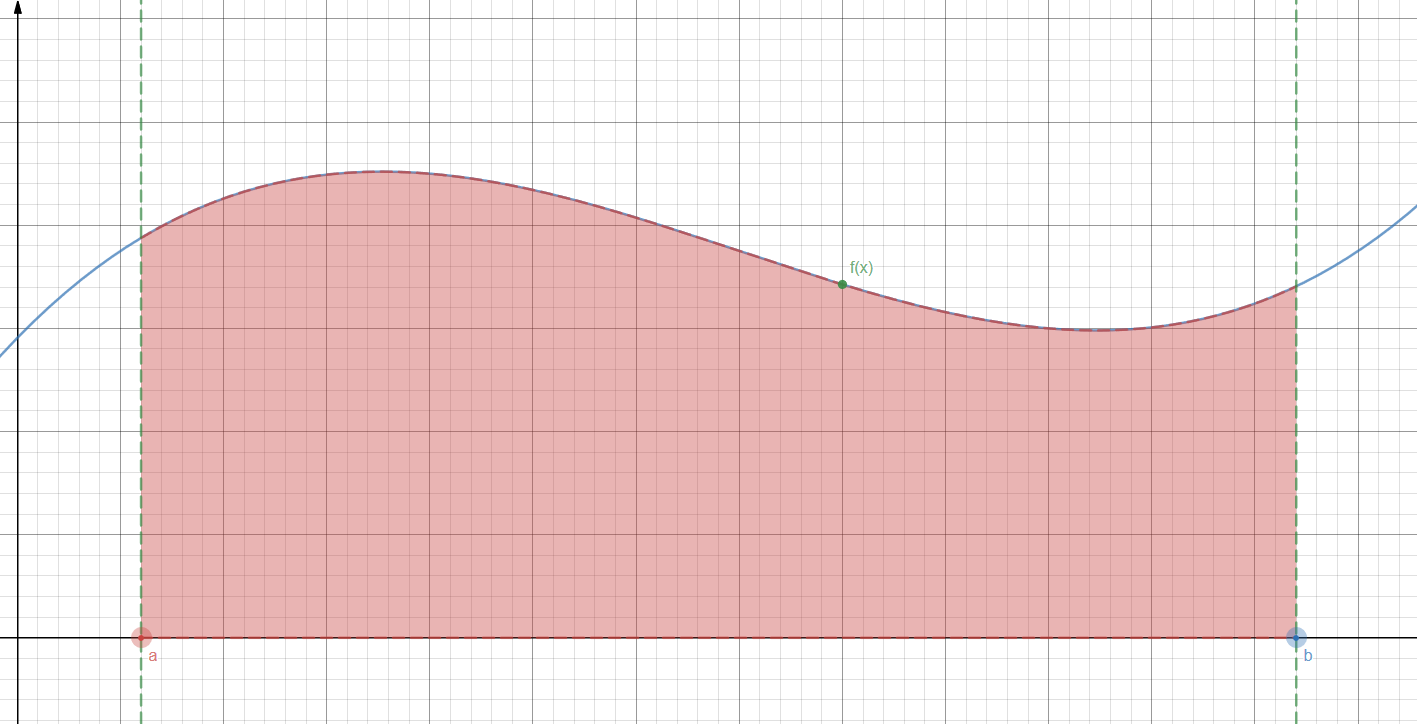
\includegraphics[width=\textwidth]{AreaUnderCurve} \\
How could we go about finding the red area, between the points \(a\) and \(b\)?

\newpage
\section{Solutions}
\begin{flalign*}
	\intertext{1.1}
	\intertext{As \(x\) limits to \(-2\), \ \(12x^2 + 5\) \ limits to \ \(12 \, (-2)^2 + 5\). So we have}
	 \lim_{x \to -2} (12x^2 + 5) &= 12 \, (-2)^2 + 5 \\
	&= 53 \asreq	
	%
	\intertext{1.2}
	\lim_{x \to a} \frac{(x + 3) \ (x - a)}{x - a} &= \lim_{x \to a} \frac{x-a}{x-a} \times \lim_{x \to a} (x + 3) \\ \\
	&= \lim_{x \to a} (1) \times \lim_{x \to a} (x + 3) \\ \\
	&= a + 3 \asreq
	%
	\intertext{1.3}
	\lim_{x \to -2} \left(12 \, \frac{x^2 - 4}{x + 2} \right) &= 12 \lim_{x \to -2} \frac{(x+2) \, (x-2)}{x+2} \\ \\
	&= 12 \lim_{x \to -2} (x-2) \\ \\
	&= 12 \times -4 \ = \ -48 \asreq
	%
	\intertext{1.4}
	\lim_{h \to 0} \frac{(6+h)^2-36}{h} &= \lim_{h \to 0} \frac{36 + 12h + h^2 - 36}{h} \\ \\
	&= \lim_{h \to 0} (12 + h) \\ \\
	&= 12 \asreq
	%
	\intertext{1.5}
	\lim_{h \to 0} \ \frac{x}{3-\sqrt{x+9}} &= \lim_{h \to 0} \frac{x \ (3 + \sqrt{x+9})}{ (3- \sqrt{x+9}) \ (3 + \sqrt{x+9})} \\ \\
	&= \lim_{h \to 0} \frac{x \ (3 + \sqrt{x + 9})}{9 - (x + 9)} \\ \\
	&= \lim_{h \to 0} - \frac{x \ (3 + \sqrt{x + 9})}{x} \\ \\
	&= \lim_{h \to 0} - (3 + \sqrt{x + 9}) \\ \\
	&= -6 \asreq
	%
	\intertext{1.6}		
	\lim_{U \to 0} \frac{1- \sqrt{1-U^2}}{U} &= \lim_{U \to 0} \frac{(1 - \sqrt{1-U^2}) \ (1 + \sqrt{1-U^2}}{U \ (1+\sqrt{1-U^2})} \\ \\
	&= \lim_{U \to 0} \ \frac{1 - 1 + U^2)}{U \ (1 + \sqrt{1-U^2})} \\ \\
	&= \lim_{U \to 0} \ \frac{U}{1+\sqrt{1-U^2}} \\ \\	
	&= \frac{0}{2} = 0 \asreq
	%
	\intertext{1.7}
	\intertext{Similarly to 1.6, }
	\lim_{\alpha \to 0} \frac{1- \sqrt{1-\alpha^3}}{\alpha^3} &= \lim_{\alpha \to 0} \ \frac{1 - (1-\alpha^3)}{a^3 \ (1 + \sqrt{1 + \alpha^3})} \\ \\
	&= \lim_{\alpha \to 0} \ \frac{1}{1 + \sqrt{1 + \alpha^3}} \\ \\
	&= \frac{1}{2} \asreq
	%
	\intertext{1.8}
	\lim_{\psi \to 0} \frac{\sqrt{a + \psi} - \sqrt{a}}{\psi} &= \lim_{\psi \to 0} \frac{(\sqrt{a + \psi} - \sqrt{a}) \ (\sqrt{a + \psi} + \sqrt{a})}{\psi \ (\sqrt{a + \psi} + \sqrt{a})} \\ \\
	&= \lim_{\psi \to 0} \ \frac{a + \psi - a}{\psi \ (\sqrt{a + \psi} + \sqrt{a})} \\ \\
	&= \lim_{\psi \to 0} \frac{1}{\sqrt{a + \psi} + \sqrt{a}} \\ \\
	&= \frac{1}{2\sqrt{a}} \\ \\
	&= \frac{\sqrt{a}}{2a} \asreq
\end{flalign*}
\end{document}

